% =====================================================================
% Med-Reasoner @ NeurIPS 2026 — Long paper (8 pages max)
% Working draft on the OFFICIAL neurips_2026.sty (in this dir).
% Compile: pdflatex paper && bibtex paper && pdflatex paper && pdflatex paper
%          (we build with tectonic on this system)
%
% Style options (see neurips_2026.sty):
%   dblblindworkshop -> double-blind workshop submission (anonymous)
%   sglblindworkshop -> single-blind workshop submission
%   final            -> camera-ready (shows author names)
%   preprint         -> arXiv-style non-anonymous preprint [DEFAULT here]
% Preprint mode shows author names for arXiv.
% =====================================================================
\documentclass{article}

\usepackage[dblblindworkshop, final]{neurips_2026}   % camera-ready (workshop)
\workshoptitle{Medical Reasoning with Vision Language Foundation Models}

\usepackage[utf8]{inputenc}
\usepackage[T1]{fontenc}
\usepackage{lmodern}   % provides T1 typewriter/roman fonts (fixes lmtt10 metric)
\usepackage{hyperref}
\usepackage{url}
\usepackage{booktabs}
\usepackage{multirow}
\usepackage{amsfonts}
\usepackage{graphicx}
\usepackage{xcolor}
\usepackage[most]{tcolorbox}

% Highlighted hypothesis box: the one-paragraph takeaway a reader can read alone.
\newtcolorbox{hypobox}[1][]{colback=blue!4, colframe=blue!45!black,
  boxrule=0.6pt, arc=2pt, left=6pt, right=6pt, top=3pt, bottom=3pt,
  title={#1}, fonttitle=\bfseries\small, coltitle=white}

\newcommand{\todo}[1]{\textcolor{red}{[TODO: #1]}}
\newcommand{\rqans}[1]{\smallskip\noindent\textbf{Answer.} #1}

\title{
\includegraphics[width=0.5\linewidth]{figures/clear_logo.png}\\[8pt]
Calibrating Medical Vision-Language\\
Reasoning Under Image Corruption}

\author{%
  Koushik Howlader\textsuperscript{1,\,*},
  Zainab Ghafoor\textsuperscript{2},
  Ushashi Bhattacharjee\textsuperscript{1}, \\
  Sayantan Chakraborty\textsuperscript{3},
  Tanusree Bhattacharjee\textsuperscript{1},
  Tirtho Roy\textsuperscript{1} \\
  \vspace{2pt} \\
  \textsuperscript{1}Iowa State University \quad
  \textsuperscript{2}Sonoma State University \quad
  \textsuperscript{3}University of Dhaka \\
  \vspace{1pt} \\
  \textsuperscript{*}Corresponding author: Koushik Howlader
  (\texttt{howlader@iastate.edu})
}

\begin{document}
\maketitle

\begin{abstract}
Vision-language models (VLMs) are now widely used to answer questions about
medical images. A known problem is that they often sound confident even when the
image does not support their answer. Earlier benchmarks test whether accuracy
drops when the image is blank or wrong, but they miss something just as important:
does the model's confidence also fall when the visual evidence is gone? Put
simply, is a VLM properly unsure when it cannot really see the image? To find out,
we test three locally run VLMs, including a medically specialized one, on two medical VQA
datasets, VQA-RAD and PathVQA, under three image conditions: intact, blank, and
mismatched. Alongside accuracy, we report calibration (expected calibration error
and reliability curves) and how often the answer stays the same when the image
changes. The results are worrying. On VQA-RAD, removing or replacing the image
lowers accuracy while mean confidence hardly moves and can even rise, so it nearly
doubles the calibration error (ECE $0.23\!\to\!0.43$). About half of all high-confidence
answers become wrong, and 48\% of answers do not change at all when the image is
swapped. The effect is even stronger on PathVQA, and, strikingly, it is worst for
the medically specialized model, which is the most overconfident of the three. Most
importantly, the models notice a blank image more easily than a believable but
wrong one, which is the more dangerous case in the clinic. We release our
evaluation harness so others can run the same calibration checks on medical VLMs.
\end{abstract}

\section{Introduction}
Vision-language models (VLMs) can now answer open questions about radiology and
pathology images, and they do so in smooth, doctor-like language. Because of this,
they are increasingly proposed as tools to help with diagnosis. In the clinic,
however, how a model shows its uncertainty matters just as much as how often it is
right. A wrong answer given with high confidence is far more dangerous than one
marked as unsure, because a clinician is more likely to trust it and act on it.

Today's hallucination benchmarks for medical VQA already test whether a model
leans on the image, usually by feeding it a blank or a wrong picture. But they
score only accuracy and refusal~\cite{halt_medvqa, medvh}. As a result, a basic
safety question stays open: when a VLM cannot actually see the right image, does
its stated confidence drop, or does it stay high? We answer this question
directly. Instead of accuracy alone, we measure calibration, which is simply the
agreement between how confident a model is and how often it is correct, and we
watch how calibration changes as we take the visual evidence away.

\begin{hypobox}[Central Hypothesis]
\small
A trustworthy medical VLM should grow \emph{less} confident when the image it needs
is blank, mismatched, or corrupted. We hypothesize that current models do the
opposite: confidence stays high even when the visual evidence is gone, so accuracy
falls but confidence does not, a calibration failure that accuracy-only benchmarks
cannot see.
\end{hypobox}

To keep the study focused, we organize it around five research questions:
\begin{itemize}
  \item \textbf{RQ1 (evidence removal).} When the image is removed or replaced,
        does the model's confidence fall as it should?
  \item \textbf{RQ2 (blank vs.\ wrong).} Does a model react differently to a blank
        image than to a believable but wrong one?
  \item \textbf{RQ3 (source).} Where does the miscalibration come from: closed
        (yes/no) questions or open ones?
  \item \textbf{RQ4 (severity).} Does confidence track a gradual loss of image
        quality, not just its sudden removal?
  \item \textbf{RQ5 (verbalized).} Is the confidence a clinician actually reads,
        the number the model states in words, any better than its internal one?
\end{itemize}
We answer all five on three locally run VLMs from different families (including a medically
specialized one) and two datasets (VQA-RAD, radiology; PathVQA, pathology), under
intact, blank, and mismatched images. For each setting we report accuracy with
expected calibration error (ECE), reliability diagrams, the high-confidence error
rate, and image-drop consistency. We release the harness so these audits are easy
to repeat.

\section{Related Work}
\paragraph{Hallucination benchmarks for medical VQA.}
HALT-MedVQA~\cite{halt_medvqa} turns VQA-RAD, PathVQA, and PMC-VQA into
multiple-choice questions with none-of-the-above and mismatched-image options, so
it can test whether models rely on the image or on training priors.
MedVH~\cite{medvh} offers a broad hallucination test that includes a ``Wrongful
Image'' task. On the detection side, semantic-entropy methods such as
VASE~\cite{vase_miccai2025} and its expanded follow-up
UniVRSE~\cite{univrse} try to catch unreliable answers. The benchmarks emphasize
task accuracy and refusal, while the detection
methods rank answers by estimated uncertainty; neither evaluates whether a model's
reported confidence remains calibrated as visual evidence is removed. That is the
gap we fill.

\paragraph{Chain-of-thought reasoning faithfulness.}
A second line of work asks whether a medical VLM's written reasoning is truly
grounded in the image. For example, \cite{eval_reasoning_faithfulness_medvlm}
separates reliance on text priors from real spatial grounding, and
S-Chain~\cite{schain} adds supervision for structured visual reasoning. These
papers ask whether the explanation matches the image. We ask a different but
related question: does the confidence attached to an answer track how much visual
evidence is available? This signal is separate from grounding faithfulness and much
cheaper to measure.

\paragraph{Confidence calibration.}
Calibration has long been studied for deep networks: expected calibration error and
reliability diagrams were popularized by Guo et al.~\cite{guo_calibration}, and
later work showed that language models can state their uncertainty in
words~\cite{lin_verbalized} and that semantic entropy captures uncertainty in
free-form generation~\cite{kuhn_semantic}. In the medical setting, recent work
reports that VLMs are often miscalibrated and
overconfident~\cite{calib_mllm_miccai, verbalized_uncertainty}, and that task
performance and image-quality judgments can be unstable under image
corruption~\cite{vlm_reliability_corruption,vlm_robustness_artifacts};
see~\cite{vlm_in_medicine_survey} for a survey. Our study
differs in two ways. Whereas \cite{vlm_reliability_corruption} uses generic
corruptions, we use a controlled removal of evidence, so a blank image and a
mismatched one separate a model's reaction to a missing image from its reaction to a
wrong one. And whereas \cite{verbalized_uncertainty} studies verbalized uncertainty
alone, we show the same overconfidence in the internal token probability and stratify
it by question type, which reveals that the well-calibrated closed questions are
exactly the ones that collapse into confident image-independent guessing.

\section{Method}
\paragraph{Datasets.} We use the test splits of VQA-RAD~\cite{vqarad}
($n{=}451$, radiology) and PathVQA~\cite{pathvqa} ($n{=}6719$, pathology). Both
mix closed (yes/no) questions with open questions about clinical images. We load
the Hugging Face mirrors identified in the bibliography. Their cards label
VQA-RAD as CC0-1.0 and PathVQA as MIT; both expose only image, question, and answer
fields, and we use no patient identifiers or private clinical records.

\paragraph{Image conditions.} For every (image, question) pair we query the model
three times. First, we use the \textbf{intact} image, the real one. Second, we use
a \textbf{blank} image, a plain gray picture of the same size that carries no
visual evidence. Third, we use a \textbf{mismatched} image, a different picture
drawn at random from the same dataset, which looks believable but is clinically
irrelevant. A faithful model should become less confident in the second and third
cases.

\paragraph{Confidence and metrics.} We decode each answer greedily and set its
confidence to the mean per-token probability of the generated text, which is the
model's own softmax confidence. We then report four numbers. Accuracy is a
normalized match to the gold answer, with some leniency for yes/no. Expected
calibration error (ECE)~\cite{guo_calibration} uses 10 equal-width bins and is
shown together with reliability diagrams. The high-confidence error rate is the fraction of answers
with confidence above 0.8 that turn out wrong. Finally, image-drop consistency is
the fraction of answers that stay exactly the same when the image is removed, which
directly measures how often the model ignores what it sees.

\paragraph{Models.} We evaluate three locally run VLMs from different model families: two
general-purpose 7B models, Qwen2.5-VL-7B-Instruct~\cite{qwen25vl} and
LLaVA-1.6-Mistral-7B~\cite{llava16}, and one medically specialized 4B model,
MedGemma-4b-it~\cite{medgemma}. All use the same decoding settings (greedy, at most
32 new tokens), and we run every question in both test splits, including the
severity sweep (RQ4) and the verbalized-confidence study (RQ5). The Qwen and LLaVA
checkpoints are Apache-2.0; MedGemma requires acceptance of Google's Health AI
Developer Foundations terms. Exact checkpoint IDs appear in the bibliography.

\section{Results}

\subsection{RQ1--RQ2: Confidence when the image is removed or replaced}
Table~\ref{tab:main} reports all three models under the three image conditions.

% ---- REAL RESULTS ----
\begin{table}[t]
\centering
\caption{Three locally run VLMs on VQA-RAD ($n{=}451$) and PathVQA ($n{=}6719$) under
three image conditions. Removing or replacing the image lowers accuracy, yet
confidence stays high and calibration error (ECE) goes up: every model stays sure
of itself exactly when it can see the least. The medically specialized model
(MedGemma) is the most overconfident of the three. \emph{Consist.} is the fraction
of answers identical to the intact-image answer.}
\label{tab:main}
\small
\setlength{\tabcolsep}{3.5pt}
\begin{tabular}{lllccccc}
\toprule
Model & Dataset & Condition & Acc $\uparrow$ & Mean conf. & ECE $\downarrow$ & Hi-conf.\ err.\ $\downarrow$ & Consist. \\
\midrule
\multirow{6}{*}{Qwen2.5-VL-7B}
 & \multirow{3}{*}{VQA-RAD}
   & Intact   & 0.554 & 0.783 & 0.229 & 0.308 & --    \\
 & & Blank    & 0.386 & 0.813 & 0.427 & 0.468 & 0.157 \\
 & & Mismatch & 0.439 & 0.806 & 0.367 & 0.463 & 0.483 \\
\cmidrule(l){2-8}
 & \multirow{3}{*}{PathVQA}
   & Intact   & 0.338 & 0.819 & 0.481 & 0.523 & --    \\
 & & Blank    & 0.246 & 0.758 & 0.513 & 0.537 & 0.315 \\
 & & Mismatch & 0.250 & 0.826 & 0.576 & 0.643 & 0.347 \\
\midrule
\multirow{6}{*}{LLaVA-1.6-7B}
 & \multirow{3}{*}{VQA-RAD}
   & Intact   & 0.439 & 0.815 & 0.375 & 0.449 & --    \\
 & & Blank    & 0.328 & 0.787 & 0.459 & 0.527 & 0.366 \\
 & & Mismatch & 0.353 & 0.813 & 0.461 & 0.545 & 0.528 \\
\cmidrule(l){2-8}
 & \multirow{3}{*}{PathVQA}
   & Intact   & 0.312 & 0.796 & 0.484 & 0.564 & --    \\
 & & Blank    & 0.224 & 0.746 & 0.521 & 0.599 & 0.193 \\
 & & Mismatch & 0.270 & 0.794 & 0.524 & 0.626 & 0.360 \\
\midrule
\multirow{6}{*}{MedGemma-4B}
 & \multirow{3}{*}{VQA-RAD}
   & Intact   & 0.548 & 0.899 & 0.351 & 0.418 & --    \\
 & & Blank    & 0.231 & 0.847 & 0.617 & 0.677 & 0.104 \\
 & & Mismatch & 0.337 & 0.886 & 0.550 & 0.653 & 0.226 \\
\cmidrule(l){2-8}
 & \multirow{3}{*}{PathVQA}
   & Intact   & 0.293 & 0.821 & 0.527 & 0.590 & --    \\
 & & Blank    & 0.139 & 0.830 & 0.691 & 0.823 & 0.078 \\
 & & Mismatch & 0.173 & 0.815 & 0.643 & 0.766 & 0.093 \\
\bottomrule
\end{tabular}
\end{table}

\rqans{(RQ1) No. Across all three models and both datasets, blanking or replacing
the image lowers accuracy, but confidence does not fall by a matching amount, so
calibration error grows. For Qwen2.5-VL, VQA-RAD ECE rises from $0.229$ to $0.427$
under blanking, and PathVQA from $0.481$ to $0.576$ under mismatch. The medically
specialized MedGemma is the worst calibrated: on PathVQA, blanking the image cuts
accuracy in half (from $0.293$ to $0.139$) while confidence actually rises
($0.821\!\to\!0.830$), pushing ECE to $0.691$ and making $82\%$ of high-confidence
answers wrong. Medical pre-training does not fix the problem; if anything, it makes
the model surer of itself.}

\rqans{(RQ2) Yes. A blank image is noticed more than a wrong one. Under a mismatched
image, every model keeps its original answer far more often than under a blank image
(for example, Qwen on VQA-RAD keeps $0.483$ of its answers under mismatch but only
$0.157$ under blank; MedGemma keeps $0.226$ under mismatch versus $0.104$ under
blank). The confidence values tell a similar but not uniform story: confidence dips
on the blank image in three of the four 7B model/dataset cells (Qwen on PathVQA
drops from $0.819$ to $0.758$), though Qwen on VQA-RAD is an exception where it rises
($0.783$ to $0.813$); under a mismatched image it stays at or above the intact level.
In other words, the models detect the absence of an
image more easily than the presence of a wrong one, which is the more dangerous case
in the clinic.}

\begin{figure}[t]
\centering
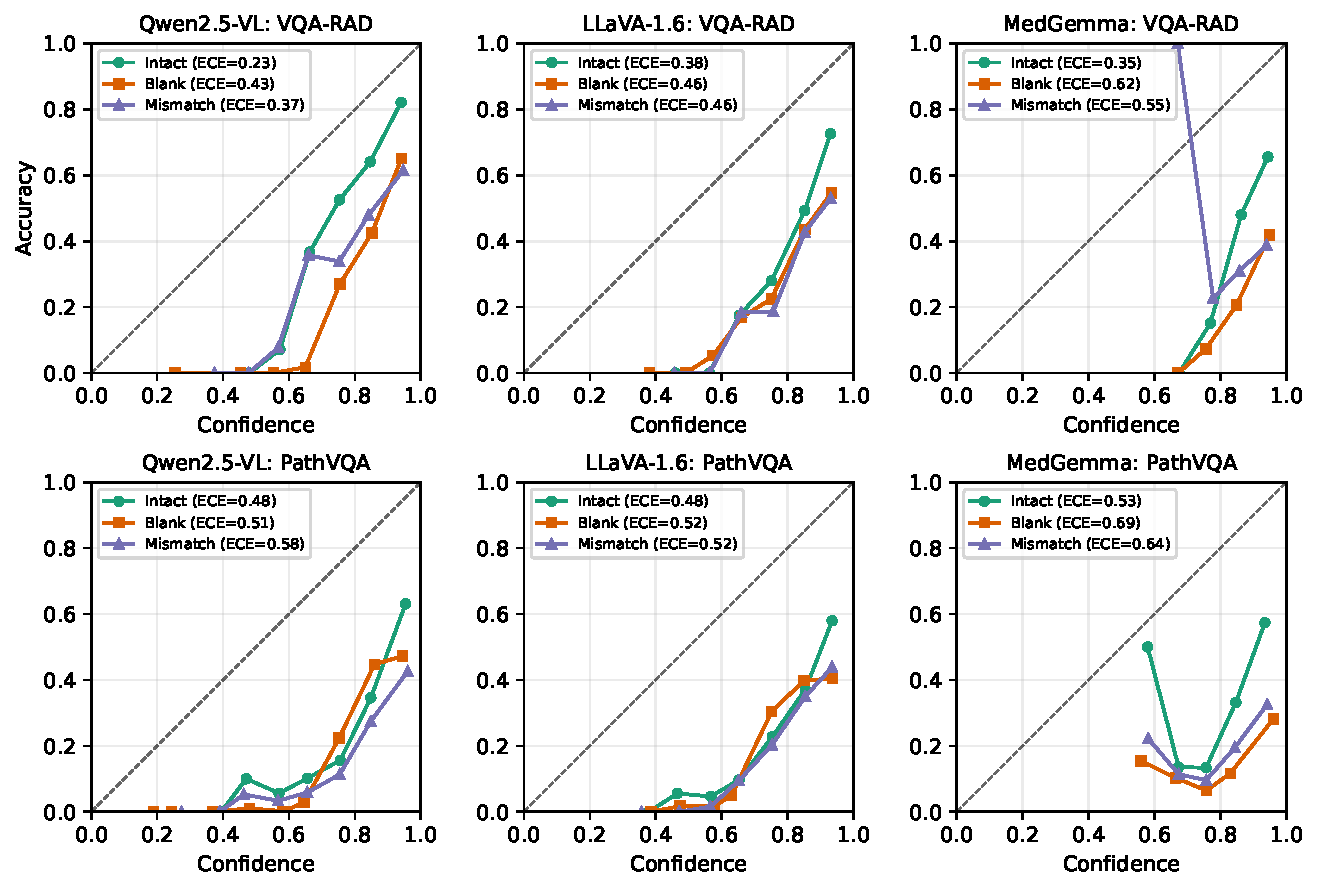
\includegraphics[width=\linewidth]{figures/reliability_three.pdf}
\caption{Reliability diagrams for all three models (columns) on both datasets
(rows: VQA-RAD top, PathVQA bottom). Points on the dashed diagonal are perfectly
calibrated, and points below it show overconfidence. Under blank and mismatched
images the curves drop further below the diagonal and ECE rises, which confirms
that confidence does not track the loss of visual evidence. The effect appears for
every model family and is worst on the harder PathVQA task and for MedGemma.}
\label{fig:reliability}
\end{figure}

Figure~\ref{fig:reliability} makes the same point visually. The intact curve sits
closest to the diagonal, while the blank and mismatched curves bow further below
it, especially on PathVQA and for MedGemma.

\subsection{RQ3: Where does the miscalibration come from?}
To see where the overconfidence lives, we split the questions into closed (yes/no)
and open groups (Table~\ref{tab:strata}).

\rqans{(RQ3) It comes from the closed questions, the ones that otherwise look most
reliable (Table~\ref{tab:strata}). With the intact image, closed questions are the
best-calibrated group, especially for Qwen2.5-VL (VQA-RAD ECE $0.05$). But once we
remove or replace the image, closed-question ECE rises sharply for every model
(on VQA-RAD, Qwen $0.05\!\to\!0.21$ and MedGemma $0.23\!\to\!0.43$ from intact to
mismatch, with the same trend on PathVQA). A bootstrap confirms this is not just
small-sample noise: for Qwen's closed questions the intact-to-mismatch ECE increase
is $+0.165$ ($95\%$ CI $[+0.083, +0.211]$). The two 7B models also fall back on a
fixed, image-independent answer: under a mismatched image they repeat their original
yes/no answer $58$ to $65\%$ of the time. MedGemma differs in one respect: it
changes its answer far more often (closed consistency only $0.18$ to $0.28$), yet it
stays just as overconfident, so its calibration is even worse. Open questions behave
differently: they are hard and overconfident in every condition (on PathVQA,
open-question accuracy is only $0.04$ with ECE above $0.70$ even on the correct
image), so their poor calibration comes from difficulty, not from missing evidence.
The dangerous pattern of confident answers that ignore the image is thus sharpest
exactly where the models otherwise look most reliable.}

\begin{table}[t]
\centering
\caption{Closed (yes/no) versus open questions for all three models. In every case,
closed-question ECE rises from the intact image to a mismatched one, while open
questions stay overconfident throughout. Consistency (\emph{Cons.}) under a
mismatched image is high for the two 7B models but lower for MedGemma, which changes
its answer more often yet is still overconfident. We show Intact and Mismatch.}
\label{tab:strata}
\small
\setlength{\tabcolsep}{4pt}
\begin{tabular}{lll cc cc c}
\toprule
& & & \multicolumn{2}{c}{Acc $\uparrow$} & \multicolumn{2}{c}{ECE $\downarrow$} & Cons. \\
\cmidrule(lr){4-5}\cmidrule(lr){6-7}\cmidrule(lr){8-8}
Model & Dataset & Type & Intact & Mism. & Intact & Mism. & Mism. \\
\midrule
\multirow{4}{*}{Qwen2.5-VL-7B}
 & \multirow{2}{*}{VQA-RAD} & Closed & 0.753 & 0.625 & 0.047 & 0.212 & 0.622 \\
 & & Open   & 0.305 & 0.205 & 0.468 & 0.563 & 0.310 \\
\cmidrule(l){2-8}
 & \multirow{2}{*}{PathVQA} & Closed & 0.634 & 0.493 & 0.254 & 0.413 & 0.629 \\
 & & Open   & 0.042 & 0.007 & 0.709 & 0.739 & 0.065 \\
\midrule
\multirow{4}{*}{LLaVA-1.6-7B}
 & \multirow{2}{*}{VQA-RAD} & Closed & 0.629 & 0.530 & 0.219 & 0.322 & 0.645 \\
 & & Open   & 0.200 & 0.130 & 0.572 & 0.635 & 0.380 \\
\cmidrule(l){2-8}
 & \multirow{2}{*}{PathVQA} & Closed & 0.599 & 0.535 & 0.253 & 0.315 & 0.578 \\
 & & Open   & 0.025 & 0.005 & 0.714 & 0.734 & 0.142 \\
\midrule
\multirow{4}{*}{MedGemma-4B}
 & \multirow{2}{*}{VQA-RAD} & Closed & 0.665 & 0.454 & 0.226 & 0.425 & 0.283 \\
 & & Open   & 0.400 & 0.190 & 0.507 & 0.707 & 0.155 \\
\cmidrule(l){2-8}
 & \multirow{2}{*}{PathVQA} & Closed & 0.503 & 0.328 & 0.349 & 0.516 & 0.175 \\
 & & Open   & 0.084 & 0.017 & 0.706 & 0.769 & 0.012 \\
\bottomrule
\end{tabular}
\end{table}

\subsection{RQ4: Does confidence track graded corruption?}
The blank and mismatch conditions take the visual evidence away all at once. To see
whether confidence tracks a gradual loss of evidence, we degrade the image step by
step for all three models, using two families of corruption: Gaussian blur (radius
$1,3,5$) and Gaussian noise ($\sigma{=}0.05,0.1,0.2$ of the pixel range). We then
recompute accuracy and mean confidence at each level (Figure~\ref{fig:severity}).

\rqans{(RQ4) No, and the pattern holds across all three models. Blur lowers accuracy,
most sharply for the medical model (MedGemma on VQA-RAD falls from $0.548$ intact to
$0.435$ at blur radius 5, its ECE rising from $0.351$ to $0.458$), yet in
every panel the confidence curve stays essentially flat and for Qwen even rises.
Noise hurts accuracy less at these levels, again with no matching drop in confidence.
Because confidence is anchored while accuracy erodes, the gap between them, and thus
ECE, widens as the image degrades for every model and dataset.}

\begin{figure}[t]
\centering
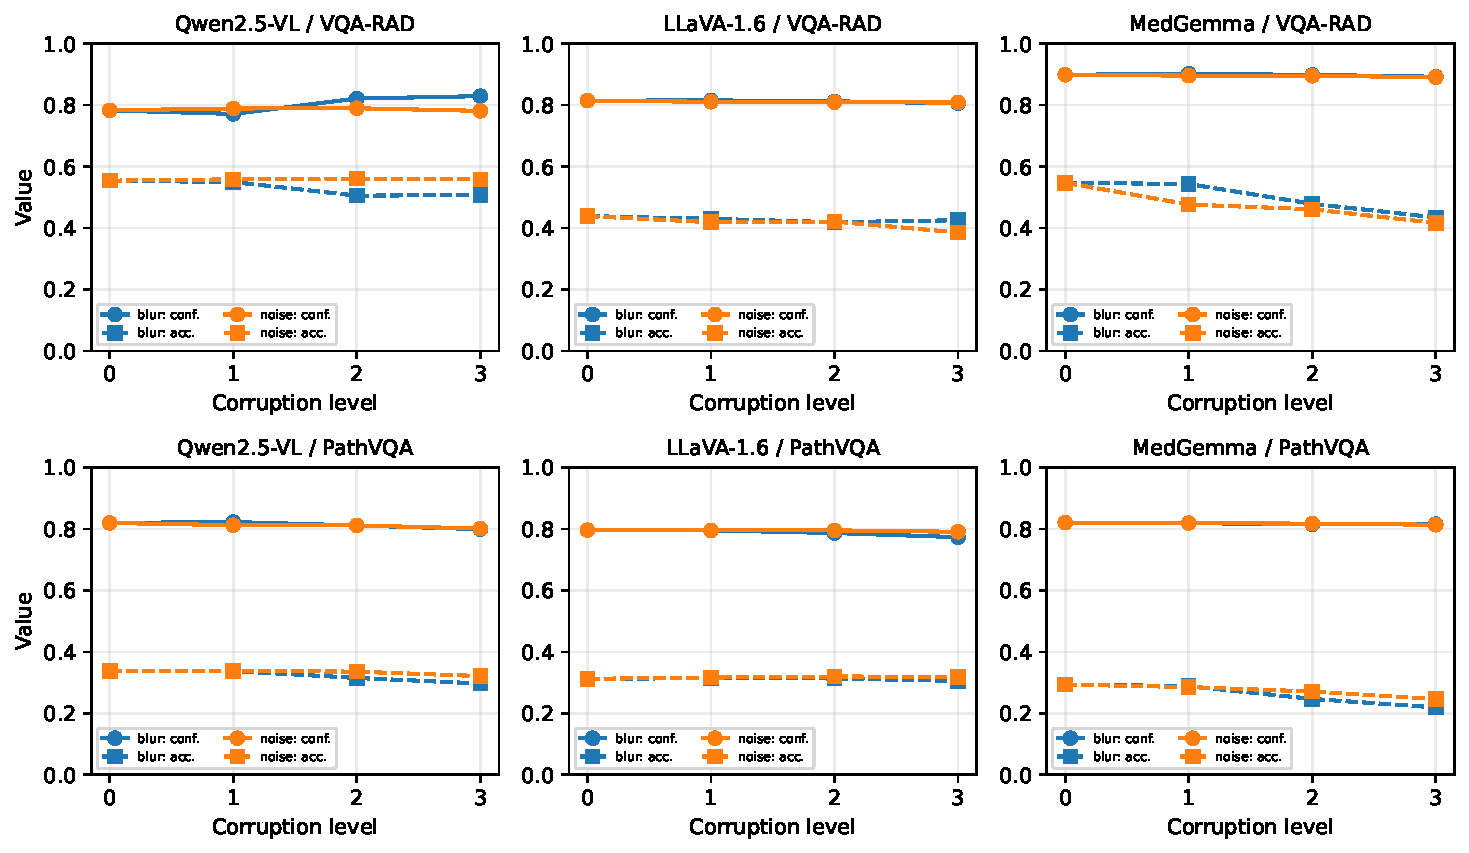
\includegraphics[width=\linewidth]{figures/severity_three.pdf}
\caption{Accuracy (dashed, squares) and mean confidence (solid, circles) for all
three models as corruption grows. The x-axis is the ordinal corruption level: $0$ is
the intact image, and levels $1$--$3$ are blur radius $1/3/5$ (blue) and noise
$\sigma{=}0.05/0.1/0.2$ (orange). In every panel confidence stays flat while
accuracy falls, so the confidence--accuracy gap, and thus ECE, widens; the effect is
strongest for the medical model (MedGemma). A faithful model's confidence curve would
fall together with accuracy.}
\label{fig:severity}
\end{figure}

\subsection{RQ5: Is verbalized confidence any better?}
Token-probability confidence is an internal number that a user never sees. A
clinician would instead read whatever confidence the model states in words. So we
run each model again with a prompt that asks it to add a line, ``Confidence:
$N$\%'', and read off the number. Table~\ref{tab:verbalized} compares the two
signals.

\rqans{(RQ5) No, and this holds for the two models that reliably comply. Qwen and
MedGemma state a parseable confidence $94$--$100\%$ of the time, and for both the
verbalized number is higher and worse calibrated than the token probability in
almost every condition; the starkest case is Qwen on VQA-RAD, which states more
confidence on a blank gray image ($0.893$) than on the real one ($0.883$), driving
verbalized ECE from $0.35$ to $0.54$. Asking for a confidence statement also inflates
the token probability itself (Qwen's VQA-RAD intact token ECE rises from $0.23$ to
$0.33$ versus the plain prompt in Table~\ref{tab:main}). LLaVA-1.6, in contrast,
emits a parseable confidence for only $13$--$26\%$ of items, usually giving no
readable number at all. So asking a medical VLM ``how sure are you?'' either makes it
more overconfident or yields nothing usable; verbalized self-assessment is not a safe
stand-in for a calibrated uncertainty estimate.}

\begin{table}[t]
\centering
\caption{Verbalized (Vrb, stated $N\%$) versus token-probability (Tok) ECE under a
prompt that asks for a confidence score; lower is better. For the two models that
reliably state a confidence (Qwen $94$--$100\%$, MedGemma ${\sim}100\%$), verbalized
confidence is worse calibrated than the token probability in almost every condition.
$^\dagger$LLaVA-1.6 emitted a parseable confidence for only $13$--$26\%$ of items, so
its verbalized column covers a small, non-representative subset and should be read
with caution.}
\label{tab:verbalized}
\small
\begin{tabular}{ll cc cc cc}
\toprule
& & \multicolumn{2}{c}{Qwen2.5-VL} & \multicolumn{2}{c}{LLaVA-1.6$^\dagger$}
  & \multicolumn{2}{c}{MedGemma} \\
\cmidrule(lr){3-4}\cmidrule(lr){5-6}\cmidrule(lr){7-8}
Dataset & Condition & Tok & Vrb & Tok & Vrb & Tok & Vrb \\
\midrule
\multirow{3}{*}{VQA-RAD} & Intact   & 0.333 & 0.351 & 0.384 & 0.568 & 0.317 & 0.329 \\
                         & Blank    & 0.474 & 0.542 & 0.450 & 0.401 & 0.580 & 0.523 \\
                         & Mismatch & 0.471 & 0.478 & 0.458 & 0.597 & 0.524 & 0.539 \\
\midrule
\multirow{3}{*}{PathVQA} & Intact   & 0.467 & 0.520 & 0.417 & 0.517 & 0.547 & 0.579 \\
                         & Blank    & 0.562 & 0.596 & 0.502 & 0.371 & 0.681 & 0.702 \\
                         & Mismatch & 0.562 & 0.561 & 0.460 & 0.603 & 0.652 & 0.679 \\
\bottomrule
\end{tabular}
\end{table}

\section{Discussion}
\paragraph{Clinical implications.} Leaderboards that report only accuracy hide the
failure we describe. The mismatched-image case is the most dangerous: a wrong scan
attached to the right patient, from a mislabeled study or a PACS error, yields a
smooth, confident, wrong answer a clinician has little reason to doubt. Our
closed-question result sharpens this: the yes/no questions that look best calibrated
on the intact image are the very ones that collapse into a confident,
image-independent guess once the image is corrupted. That medical pre-training does
not help, and that the medical model is the most overconfident, warns against
assuming a specialized model is safer.
\paragraph{Toward mitigation.} The audit points to a few cheap safeguards. First,
report calibration, not just accuracy: ECE and the high-confidence error rate under
blank and mismatched images should go alongside any medical VQA accuracy claim.
Second, do not trust verbalized confidence, since it is worse than the already poor
token probability. Third, use simple consistency checks: because answers rarely
change under a mismatched image (up to $0.63$ for closed questions), testing whether
the answer moves when the image is perturbed can flag responses that ignore it. We
leave calibration-aware fine-tuning and post-hoc methods to future work.
\paragraph{Limitations.} Our study has clear limits. It covers three locally run VLMs (two
7B general models and one 4B medical model); larger models, and other
medically specialized ones such as LLaVA-Med, may calibrate differently. We use two
datasets (radiology
and pathology) and greedy decoding, so sampling-based confidence and other
modalities remain untested. Our confidence score is a mean over generated tokens,
which could be refined, for instance by averaging only over the answer span. Finally,
ECE with 10 bins on small splits (VQA-RAD has only 451
items) can be noisy, so we report a bootstrap interval for the key closed-question
result and otherwise stress effects that hold across both datasets and all three
models.

\section{Conclusion}
We audited three locally run VLMs on radiology and pathology VQA, and we found a
consistent problem: their confidence does not fall when the visual evidence they
need is removed or replaced. Accuracy drops, yet confidence stays high, so
calibration error rises sharply and many confident answers are wrong. The failure
holds across model families and, tellingly, is worst for the medically specialized
model. Most worrying for clinical use, the models react more to a blank image than
to a believable but wrong one, which is exactly the case where a confidently
incorrect answer is most likely to be trusted. The same overconfidence grows
steadily as corruption increases, most sharply for the medical model, and the
verbalized confidence a clinician would actually read is even worse calibrated than
the internal signal for the models that state one at all. The failure is also
concentrated in the closed questions that otherwise look most reliable. These failures are invisible to accuracy-only benchmarks, which is
why we argue that calibration and image-drop checks should be a routine part of
testing medical VLMs. We release our harness so these audits are easy to reproduce.

\bibliographystyle{plainnat}
\bibliography{references}

\newpage
\section*{NeurIPS Paper Checklist}

\begin{enumerate}

\item {\bf Claims}
    \item[] Question: Do the main claims made in the abstract and introduction accurately reflect the paper's contributions and scope?
    \item[] Answer: \answerYes{}
    \item[] Justification: The abstract and Introduction state the central claim---that confidence fails to fall when visual evidence is removed, replaced, or corrupted, so calibration error rises---and the Results (RQ1--RQ5) and Tables~\ref{tab:main}--\ref{tab:verbalized} support exactly these claims, with scope limited to the three evaluated models and two datasets.

\item {\bf Limitations}
    \item[] Question: Does the paper discuss the limitations of the work performed by the authors?
    \item[] Answer: \answerYes{}
    \item[] Justification: The Discussion contains a dedicated Limitations paragraph covering the three-model/two-dataset scope, greedy decoding, the mean-over-tokens confidence proxy, and small-split ECE noise (for which a bootstrap interval is reported).

\item {\bf Theory assumptions and proofs}
    \item[] Question: For each theoretical result, does the paper provide the full set of assumptions and a complete (and correct) proof?
    \item[] Answer: \answerNA{}
    \item[] Justification: The paper is an empirical audit and contains no theoretical results or proofs.

    \item {\bf Experimental result reproducibility}
    \item[] Question: Does the paper fully disclose all the information needed to reproduce the main experimental results of the paper to the extent that it affects the main claims and/or conclusions of the paper (regardless of whether the code and data are provided or not)?
    \item[] Answer: \answerYes{}
    \item[] Justification: The Setup describes the exact models, datasets, image conditions, decoding settings (greedy, at most 32 new tokens), confidence definition, and ECE binning; the evaluation harness is released, and all datasets and model checkpoints are public.

\item {\bf Open access to data and code}
    \item[] Question: Does the paper provide open access to the data and code, with sufficient instructions to faithfully reproduce the main experimental results, as described in supplemental material?
    \item[] Answer: \answerYes{}
    \item[] Justification: We release the evaluation harness (model-agnostic inference, scoring, stratification, bootstrap CIs, and plotting scripts) with usage instructions; both datasets (VQA-RAD, PathVQA) and all three model checkpoints are publicly available on the Hugging Face Hub as identified in the bibliography.

\item {\bf Experimental setting/details}
    \item[] Question: Does the paper specify all the training and test details (e.g., data splits, hyperparameters, how they were chosen, type of optimizer) necessary to understand the results?
    \item[] Answer: \answerYes{}
    \item[] Justification: No training is performed; the Setup specifies the test splits (VQA-RAD $n{=}451$, PathVQA $n{=}6719$), the three image conditions, greedy decoding with at most 32 new tokens, and the 10-bin ECE used throughout.

\item {\bf Experiment statistical significance}
    \item[] Question: Does the paper report error bars suitably and correctly defined or other appropriate information about the statistical significance of the experiments?
    \item[] Answer: \answerYes{}
    \item[] Justification: For the key RQ3 result we report a bootstrap 95\% confidence interval (5000 resamples of items with replacement, percentile interval) on the intact-to-mismatch ECE increase for closed questions; the interval excludes zero. Other metrics are computed on the full test splits.

\item {\bf Experiments compute resources}
    \item[] Question: For each experiment, does the paper provide sufficient information on the computer resources (type of compute workers, memory, time of execution) needed to reproduce the experiments?
    \item[] Answer: \answerYes{}
    \item[] Justification: All experiments are inference only (no training). Each model/dataset run used a single NVIDIA A100 GPU; the heaviest runs (the full severity sweep over PathVQA, seven conditions $\times$ 6719 items) take on the order of hours, and total compute is modest.

\item {\bf Code of ethics}
    \item[] Question: Does the research conducted in the paper conform, in every respect, with the NeurIPS Code of Ethics \url{https://neurips.cc/public/EthicsGuidelines}?
    \item[] Answer: \answerYes{}
    \item[] Justification: The work uses publicly available, de-identified medical VQA datasets and performs inference only; it involves no human subjects and is aimed at improving the safety and reliability of medical VLMs.

\item {\bf Broader impacts}
    \item[] Question: Does the paper discuss both potential positive societal impacts and negative societal impacts of the work performed?
    \item[] Answer: \answerYes{}
    \item[] Justification: The Discussion (Clinical implications) describes the positive impact---surfacing a safety-relevant calibration failure invisible to accuracy-only benchmarks and recommending cheap safeguards---and the motivating negative scenario of confidently wrong answers on degraded or mismatched medical images.

\item {\bf Safeguards}
    \item[] Question: Does the paper describe safeguards that have been put in place for responsible release of data or models that have a high risk for misuse (e.g., pre-trained language models, image generators, or scraped datasets)?
    \item[] Answer: \answerNA{}
    \item[] Justification: We release only an evaluation harness (analysis code); no new model, generator, or scraped dataset with misuse risk is released.

\item {\bf Licenses for existing assets}
    \item[] Question: Are the creators or original owners of assets (e.g., code, data, models), used in the paper, properly credited and are the license and terms of use explicitly mentioned and properly respected?
    \item[] Answer: \answerYes{}
    \item[] Justification: All datasets and models are cited, and their licenses/terms are noted in the bibliography (VQA-RAD CC0-1.0, PathVQA MIT, Qwen2.5-VL and LLaVA-1.6 Apache-2.0, MedGemma under the Health AI Developer Foundations terms).

\item {\bf New assets}
    \item[] Question: Are new assets introduced in the paper well documented and is the documentation provided alongside the assets?
    \item[] Answer: \answerYes{}
    \item[] Justification: The only new asset is the evaluation harness, which is released with a README describing dependencies, the datasets/models to download, and exact commands to reproduce each experiment.

\item {\bf Crowdsourcing and research with human subjects}
    \item[] Question: For crowdsourcing experiments and research with human subjects, does the paper include the full text of instructions given to participants and screenshots, if applicable, as well as details about compensation (if any)?
    \item[] Answer: \answerNA{}
    \item[] Justification: The paper does not involve crowdsourcing or research with human subjects; it uses existing public datasets.

\item {\bf Institutional review board (IRB) approvals or equivalent for research with human subjects}
    \item[] Question: Does the paper describe potential risks incurred by study participants, whether such risks were disclosed to the subjects, and whether Institutional Review Board (IRB) approvals (or an equivalent approval/review based on the requirements of your country or institution) were obtained?
    \item[] Answer: \answerNA{}
    \item[] Justification: The paper does not involve human subjects, so no IRB approval is required.

\item {\bf Declaration of LLM usage}
    \item[] Question: Does the paper describe the usage of LLMs if it is an important, original, or non-standard component of the core methods in this research? Note that if the LLM is used only for writing, editing, or formatting purposes and does \emph{not} impact the core methodology, scientific rigor, or originality of the research, declaration is not required.
    \item[] Answer: \answerNA{}
    \item[] Justification: The vision-language models in this paper are the objects of evaluation, not tools used to develop the methodology; no LLM is an important, original, or non-standard component of the core method.

\end{enumerate}


\end{document}
